\documentclass{beamer}
\usepackage{ctex, hyperref}
\usepackage[T1]{fontenc}

% other packages
\usepackage{latexsym,amsmath,xcolor,multicol,booktabs,calligra}
\usepackage{graphicx,pstricks,listings,stackengine}

\author{Your Name / Team Name}
\title{NoHeadcountSystem}
\subtitle{High-Performance Cryptocurrency HFT System}
\institute{Your Institution / Department}
\date{\today}
\usepackage{CUHKSZ}

% defs
\def\cmd#1{\texttt{\color{red}\footnotesize $\backslash$#1}}
\def\env#1{\texttt{\color{blue}\footnotesize #1}}
\xdefinecolor{cuhksz1}{rgb}{0.457,0.0585,0.42578}      %RGB(117,15,109)
\xdefinecolor{cuhksz2}{rgb}{0.86328,0.63671875,0}      %RGB(221,163,0)
\xdefinecolor{cuhksz3}{rgb}{0.953125,0.87109,0.6875}   %RGB(244,223,176)

\definecolor{deepred}{rgb}{0.6,0,0}

\lstset{
    basicstyle=\ttfamily\small,
    keywordstyle=\bfseries\color{cuhksz1},
    emphstyle=\ttfamily\color{deepred},
    stringstyle=\color{cuhksz2},
    numbers=left,
    numberstyle=\small\color{cuhksz3},
    rulesepcolor=\color{red!20!green!20!blue!20},
    frame=shadowbox,
}

\begin{document}

\kaishu
\begin{frame}
    \titlepage
    \begin{figure}[htpb]
        \begin{center}
            
\includegraphics[width=0.3\linewidth]{pic/CUHKSZ-Logo.pdf}
        \end{center}
    \end{figure}
\end{frame}

\begin{frame}
    \tableofcontents[sectionstyle=show,subsectionstyle=show/shaded/hide,subsubsectionstyle=show/shaded/hide]
\end{frame}

\section{Team Division}

\begin{frame}{Team Division}
    \begin{table}[htpb]
        \centering
        \caption{Project Task Allocation}
        \label{tab:team}
        \begin{tabular}{c|c}
            \toprule
            \textbf{Team Member}  & \textbf{Contribution} \\
            \midrule
            Mo Yunjie & Strategies, System Outline, Report  \\
            Li Taiyan & Infrastructure, OMS, GUI \\
            Guo Xiaoyou & Event-Driven Backtesting \\
            Huang Yujin & Risk Management, TCA \\
            \bottomrule
        \end{tabular}
    \end{table}
\end{frame}

\section{Project Background \& Introduction}

\begin{frame}{Project Background \& Introduction}
    \begin{itemize}
        \item \textbf{System Positioning}: A High-Frequency Trading (HFT) system tailored for futures and cryptocurrencies.
        \item \textbf{Core Features}:
        \begin{itemize}
            \item \textbf{Modular Design}: Decoupled infrastructure, strategies, risk management, and backtesting components.
            \item \textbf{Event-Driven}: Non-blocking data and instruction routing based on a unified event bus.
            \item \textbf{Seamless Switching}: One-click switch between simulated matching (SIM) and Binance Spot Testnet (BINANCE).
        \end{itemize}
        \item \textbf{Tech Stack}: Python, Numba (High-performance computing), \texttt{uv} (Fast dependency management).
    \end{itemize}
\end{frame}

\section{Core Architecture}

\begin{frame}{Core Architecture \& Data Flow}
    \begin{itemize}
        \item \textbf{System Bus}: Modules are fully decoupled using the \texttt{EventEngine}.
        \item \textbf{Data Pipeline}:
        \begin{enumerate}
            \item \textbf{Tick}: Market data enters the system.
            \item \textbf{Strategy}: Listens to Ticks and generates a \texttt{Signal}.
            \item \textbf{OMS (Order Management)}: Converts Signals into standardized \texttt{Order}s.
            \item \textbf{RMS (Risk Management)}: Intercepts and validates orders (limits, exposure).
            \item \textbf{Gateway}: Routes to the target exchange or simulator.
            \item \textbf{Trade}: Execution reports flow back via the event bus to update all modules.
        \end{enumerate}
    \end{itemize}
\end{frame}

\section{Infrastructure}

\begin{frame}{Infrastructure Layer}
    \begin{itemize}
        \item \textbf{Gateway Connection}:
        \begin{itemize}
            \item \texttt{BinanceTestnetGateway}: Connects to Binance Spot Testnet for live testing.
            \item \texttt{SimulatedGateway}: Local simulated matching engine for safe debugging.
        \end{itemize}
        \item \textbf{Unified Data Models}: Standardized \texttt{TickData}, \texttt{Signal}, \texttt{OrderData}, \texttt{TradeData}.
        \item \textbf{Order Management System (OMS)}:
        \begin{itemize}
            \item Bridges the strategy end (signals) and the channel end (orders).
            \item Automatically tracks order status updates and maintains the signal-to-order mapping lifecycle.
        \end{itemize}
    \end{itemize}
\end{frame}

\section{Strategies \& Execution Layer}

\begin{frame}{Strategies \& Execution Layer}
    \begin{itemize}
        \item \textbf{Strategy Base (\texttt{base.py})}: Standardized interfaces where strategies only emit signals without placing orders directly, keeping responsibilities single and clean.
        \item \textbf{Featured Strategy: \texttt{FeeAwareStatArbStrategy} (\texttt{dca.py})}
        \begin{itemize}
            \item \textbf{Statistical Arbitrage}: Uses an Exponential Moving Average (EMA) to calculate micro-price deviations.
            \item \textbf{Fee-Aware Logic}: Entries require the potential profit to strictly exceed double taker fees (\texttt{taker\_fee $\times$ 2}) plus a target profit rate.
            \item \textbf{Dollar-Cost Averaging (DCA)}: Dynamically adds to losing positions with strict step rates to lower the average cost.
            \item \textbf{Smart Order Splitting}: Automatically splits position adjustments into legal \texttt{CLOSE} and \texttt{OPEN} offset signals.
        \end{itemize}
    \end{itemize}
\end{frame}

\begin{frame}{Arbitrage Strategy Results}
    \begin{columns}
        \begin{column}{0.55\textwidth}
            \textbf{In-Sample Equity Curve}
            \begin{figure}[htpb]
                \centering
                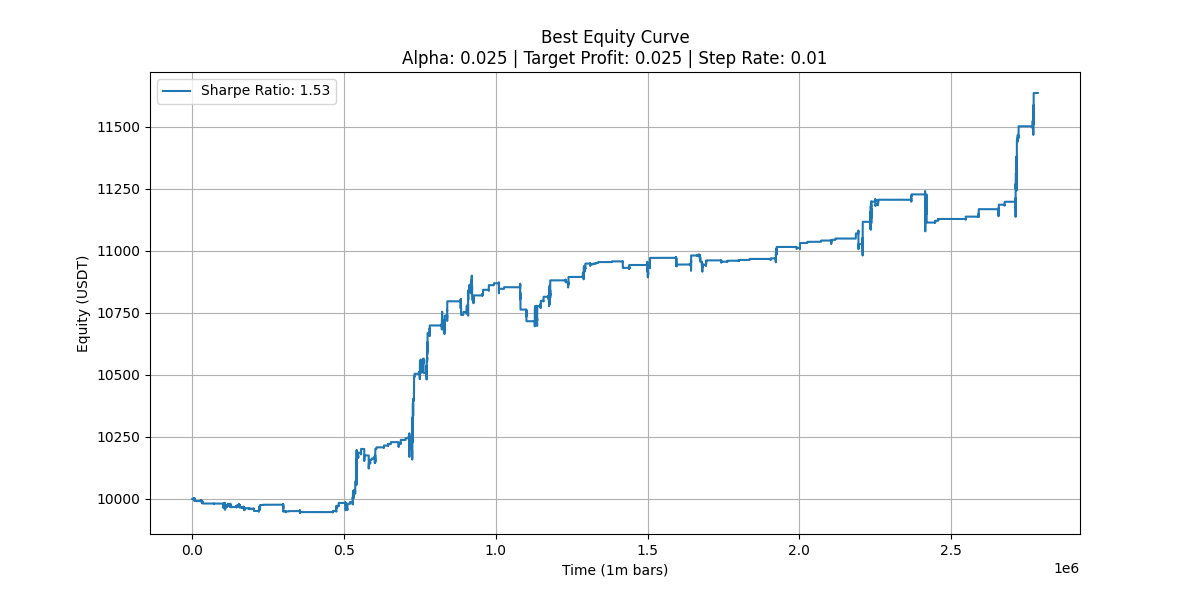
\includegraphics[width=\linewidth]{pic/equity_curve.png}
            \end{figure}
        \end{column}
        \begin{column}{0.45\textwidth}
            \textbf{Out-of-Sample Metrics}
            \begin{itemize}
                \item Initial Capital: 10000.0
                \item Realized PnL: 66.20
                \item Turnover: 9770.01
                \item End Position: 0.0
                \item Closed Trades: 8
                \vspace{0.2cm}
                \item \textbf{Annualized Return}: 0.66\%
                \item \textbf{Annualized Volatility}: 0.47\%
                \item \textbf{Sharpe Ratio}: 1.42
                \item \textbf{Max Drawdown}: 0.37\%
            \end{itemize}
        \end{column}
    \end{columns}
\end{frame}

\section{Risk Management}

\begin{frame}{Risk Management Center (RMS)}
    \begin{itemize}
        \item \textbf{Real-time Interception System}: Acts as the last line of defense before orders are dispatched to the exchange (\texttt{manager.py}).
        \item \textbf{Core Risk Rules}:
        \begin{itemize}
            \item \textbf{Max Order Volume} (\texttt{max\_order\_volume}): Prevents fat-finger errors and extreme anomalies.
            \item \textbf{Max Net Position} (\texttt{max\_symbol\_position}): Controls unilateral exposure and inventory risks.
        \end{itemize}
        \item \textbf{Dynamic Scalability}: The architecture allows for hot-plugging of new risk validation rules without altering the core pipeline.
    \end{itemize}
\end{frame}

\section{Backtest Engine}

\begin{frame}{High-Performance Backtest Engine}
    \begin{itemize}
        \item \textbf{Core Driver}: Numba-accelerated K-line backtesting core (\texttt{exchange.py} \& \texttt{loop.py}).
        \item \textbf{Matching Mechanism}:
        \begin{itemize}
            \item \textbf{Bar-Level Dual Sweep}: Simulates intra-bar volatility by scanning triggering limits through High and Low prices sequentially.
            \item \textbf{Aggressive Limit Conversion}: Automatically converts marketable limit orders to market orders.
        \end{itemize}
        \item \textbf{Accurate Accounting}:
        \begin{itemize}
            \item Built-in Taker/Maker commission models.
            \item Real-time maintenance of positions, cost prices, realized/unrealized PnL, and capital turnover.
        \end{itemize}
    \end{itemize}
\end{frame}

\section{Dashboard \& Deployment}

\begin{frame}{Dashboard \& GUI}
    \begin{itemize}
        \item \textbf{GUI Monitor}: Real-time metrics, dynamic grids for orders/trades/ticks, and event timeline tracking.
        \item \textit{Supports headless mode (\texttt{ENABLE\_GUI=0}) for cloud server deployment.}
    \end{itemize}
    \vspace{-0.2cm}
    \begin{figure}[htpb]
        \centering
        \includegraphics[width=0.95\linewidth]{pic/gui.png}
    \end{figure}
\end{frame}

\begin{frame}{Quick Start}
    \begin{itemize}
        \item \textbf{Minimal Dependencies}: Uses \texttt{uv} (Rust-based Python package manager) for instant environment syncing (\texttt{uv sync}).
        \item \textbf{Config-Driven (\texttt{.env})}:
        \begin{itemize}
            \item \texttt{TRADING\_MODE=SIM/BINANCE} for one-click environment switches.
            \item Centralized configuration for API keys, proxies, and strategy parameters.
        \end{itemize}
        \item \textbf{One-Command Run}: \texttt{uv run src/main.py} automatically initializes all modules and starts the event loop.
    \end{itemize}
\end{frame}

\section{Conclusion \& Future Work}

\begin{frame}{Conclusion \& Future Work}
    \begin{itemize}
        \item \textbf{System Advantages}:
        \begin{itemize}
            \item Clear isolation of responsibilities (signals decoupled from orders).
            \item High extensibility for new exchanges and strategies.
            \item Consistent logic between backtesting and live trading.
        \end{itemize}
        \item \textbf{Future Extensions}:
        \begin{itemize}
            \item Integrate more exchange gateways (e.g., OKX, Bybit).
            \item Introduce Machine Learning models for alpha signal prediction.
            \item Enhanced backtest charting and detailed attribution reports.
        \end{itemize}
    \end{itemize}
\end{frame}

\begin{frame}
    \begin{center}
        {\Huge\calligra Q\&A / Thank You!}
    \end{center}
\end{frame}

\end{document}
